
%{{第二十五回}}{第二十五回}}

\chapter{魇魔法叔嫂逢五鬼 通灵玉蒙蔽遇双真}\label{part0029_split_000.htmlux5cux23calibre_pb_0}

{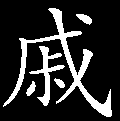
\includegraphics[width=3mm]{../Images/00005}有缘的,推不开;知心的,死不改。纵然是通灵神玉也遭尘败。梦里徘徊,醒后疑猜,时时兜底上心来。怕人窥破笑盈腮,独自无言偷打咳。这的是、前生造定今生债。}

话说红玉情思缠绵,忽朦胧睡去,见贾芸要拉他,却回身一跑,被门槛子绊了一跤,唬醒过来,方知是梦。因此翻来覆去,一夜无眠。至次日天明,方才起来,就有几个丫头来会他去打扫屋子地,提洗脸水。这红玉也不梳洗,向镜中胡乱挽了一挽头发,洗了洗手,腰内束了一条汗巾子,便来扫地。

谁知宝玉昨儿见了红玉,也就留了心。若要直点名唤他来使用,一则怕袭人等寒心;{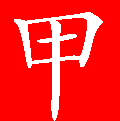
\includegraphics[width=3mm]{../Images/00002}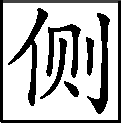
\includegraphics[width=3mm]{../Images/00011}\footnotesize \kaishu 是宝玉心中想,不是袭人拈酸。}二则又不知红玉是何等行为,若好还罢了,{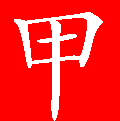
\includegraphics[width=3mm]{../Images/00002}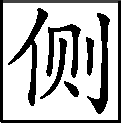
\includegraphics[width=3mm]{../Images/00011}\footnotesize \kaishu 不知``好''字是如何讲?答曰:在``何等行为''四字上看便知,玉兄每情不情,况有情者乎?}若不好起来,那时倒不好退送的。因此心中闷闷的,一早起来也不梳洗,只坐着出神。一时下了窗子,隔着纱屉子,向外看的真切,只见好几个丫头在那里扫地,都擦胭抹粉,簪花插柳的,{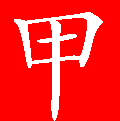
\includegraphics[width=3mm]{../Images/00002}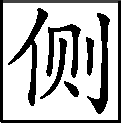
\includegraphics[width=3mm]{../Images/00011}\footnotesize \kaishu 八字写尽蠢鬟,是为衬红玉,亦如用豪贵人家浓妆艳饰插金戴银的衬宝钗、黛玉也。}独不见昨儿那一个。宝玉便靸了鞋,晃出了房门,只装着看花儿,这里瞧瞧,那里望望,{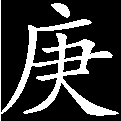
\includegraphics[width=3mm]{../Images/00004}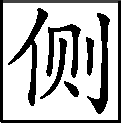
\includegraphics[width=3mm]{../Images/00011}\footnotesize \kaishu 文字有层次。}一抬头,只见西南角上游廊底下栏杆外,似有一个人在那里倚着,却恨面前有一株海棠花遮着,看不真切。{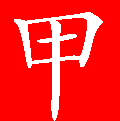
\includegraphics[width=3mm]{../Images/00002}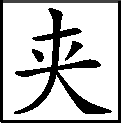
\includegraphics[width=3mm]{../Images/00012}\footnotesize \kaishu 余所谓此书之妙,皆从诗词句中翻出者,皆系此等笔墨也。试问观者,此非``隔花人远天涯近''乎?可知上几回非余妄拟也。}只得又转了一步,仔细一看,可不是昨儿的那个丫头在那里出神?待要迎上去,又不好去的。正想着,忽见碧痕来催他洗脸,只得进去了。不在话下。

却说红玉正自出神,忽见袭人招手叫他,{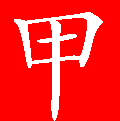
\includegraphics[width=3mm]{../Images/00002}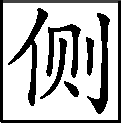
\includegraphics[width=3mm]{../Images/00011}\footnotesize \kaishu 此处方写出袭人来,是衬贴法。}只得走来。袭人道:``你到林姑娘那里去,把他们的喷壶借来使使,我们的还没有收拾了来呢。''红玉答应了,便往潇湘馆去。正走上翠烟桥,抬头一望,只见山坡上高处都拦着帏幕,方想起今儿有匠人在里头种树。因转身一望,只见那边远远的一簇人在那里掘土,贾芸正坐在山子石上。红玉待要过去,又不敢过去,只得闷闷的向潇湘馆取了喷壶回来,无精打彩,自向房内倒着去。众人只说他一时身上不快,都不理论。{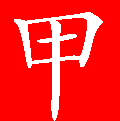
\includegraphics[width=3mm]{../Images/00002}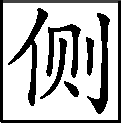
\includegraphics[width=3mm]{../Images/00011}\footnotesize \kaishu 文字到此一顿,狡猾之甚。}

展眼过了一日,{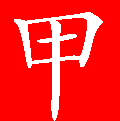
\includegraphics[width=3mm]{../Images/00002}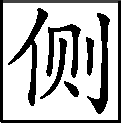
\includegraphics[width=3mm]{../Images/00011}\footnotesize \kaishu 必云``展眼过了一日''者,是反衬红玉``捱一刻似一夏''也,知乎?}原来次日就是王子腾夫人的寿诞,那里原打发人来请贾母王夫人的,王夫人见贾母不去,自己也便不去了。{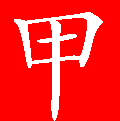
\includegraphics[width=3mm]{../Images/00002}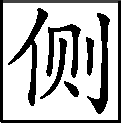
\includegraphics[width=3mm]{../Images/00011}\footnotesize \kaishu 所谓一笔两用也!}倒是薛姨妈同凤姐儿并贾家三\href{../Text/part0029_split_000.html\#lnkback_1_a}{\textsuperscript{①}}个姊妹、宝钗、宝玉一齐都去了,至晚方回。

且说王夫人见贾环下了学,便命他来抄个《金刚咒》{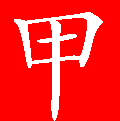
\includegraphics[width=3mm]{../Images/00002}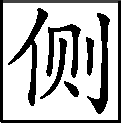
\includegraphics[width=3mm]{../Images/00011}\footnotesize \kaishu 用《金刚咒》引五鬼法。}唪诵。那贾环在王夫人炕上坐了,命人点上灯,拿腔作势的抄写。{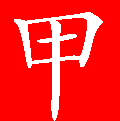
\includegraphics[width=3mm]{../Images/00002}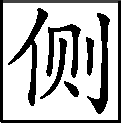
\includegraphics[width=3mm]{../Images/00011}\footnotesize \kaishu 小人乍得意者齐来一玩。}一时叫彩云倒茶来,一时又叫玉钏儿来剪剪灯花,一时又说金钏儿挡了灯影。众丫头们素日厌恶他,都不答理。只有彩霞还和他合的来,{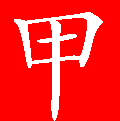
\includegraphics[width=3mm]{../Images/00002}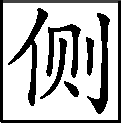
\includegraphics[width=3mm]{../Images/00011}\footnotesize \kaishu 暗中又伏一风月之隙。}倒了一钟茶来递与他。见王夫人和人说话儿,便悄悄的向贾环说道:``你安些分罢,何苦讨这个厌呢。''贾环道:``我也知道了,你别哄我。如今你和宝玉好,把我不答理,我也看出来了。''彩霞咬着嘴唇,向贾环头上戳了一指头,说道:``没良心的!才是狗咬吕洞宾,不识好人心。''{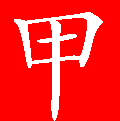
\includegraphics[width=3mm]{../Images/00002}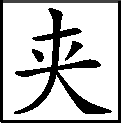
\includegraphics[width=3mm]{../Images/00012}\footnotesize \kaishu 风月之情,皆系彼此业障所牵。虽云``惺惺惜惺惺'',但亦从业障而来。蠢妇配才郎,世间固不少,然俏女慕村夫者尤多,所谓业障牵魔,不在才貌之论。 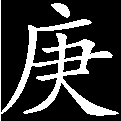
\includegraphics[width=3mm]{../Images/00004}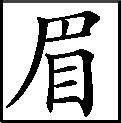
\includegraphics[width=3mm]{../Images/00010}\footnotesize \kaishu 此等世俗之言,亦因人而用,妥极当极!壬午孟夏,雨窗。畸笏。}

两人正说着,只见凤姐来了,拜见过王夫人。王夫人便一长一短的问他,今儿是那几位堂客在那里,戏文如何,酒席好歹等话。说了不多几句,宝玉也来了,进门见了王夫人,不过规规矩矩说了几句话,{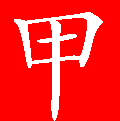
\includegraphics[width=3mm]{../Images/00002}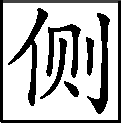
\includegraphics[width=3mm]{../Images/00011}\footnotesize \kaishu 是大家子弟模样。}便命人除去抹额,脱了袍服,拉了靴子,便一头滚在王夫人怀内。{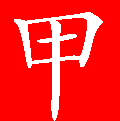
\includegraphics[width=3mm]{../Images/00002}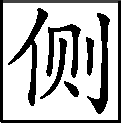
\includegraphics[width=3mm]{../Images/00011}\footnotesize \kaishu 余几几失声哭出。}王夫人便用手满身满脸摩挲抚弄他,{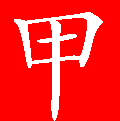
\includegraphics[width=3mm]{../Images/00002}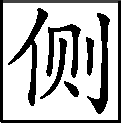
\includegraphics[width=3mm]{../Images/00011}\footnotesize \kaishu 普天下幼年丧母者齐来一哭。}宝玉也搬着王夫人的脖子说长道短的。{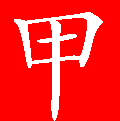
\includegraphics[width=3mm]{../Images/00002}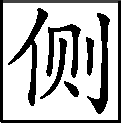
\includegraphics[width=3mm]{../Images/00011}\footnotesize \kaishu 慈母娇儿写尽矣。}王夫人道:``我的儿,你又吃多了酒,脸上滚热。你还只是揉搓,一会闹上酒来。还不在那里静静的倒一会子呢。''说着,便叫人拿个枕头来。宝玉听了便下来,在王夫人身后倒下,又叫彩霞来替他拍着。宝玉便和彩霞说笑,只见彩霞淡淡的不大答理,两眼睛只向贾环处看。宝玉便拉他的手笑道:``好姐姐,你也理我一理儿呢。''彩霞夺了手道:``再闹,我就嚷了。''

二人正说,原来贾环听的见,素日原恨宝玉,如今又见他和彩霞厮闹,心中越发按不下这口毒气。虽不敢明言,却每每暗中算计,{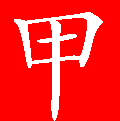
\includegraphics[width=3mm]{../Images/00002}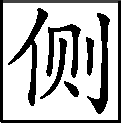
\includegraphics[width=3mm]{../Images/00011}\footnotesize \kaishu 已伏金钏回矣。}只是不得下手。今儿相离甚近,便要用蜡灯里的滚油烫他一下。因而故意装作失手,把那一盏油汪汪的蜡灯向宝玉脸上只一推。只听宝玉``嗳哟''了一声,满屋人都唬一跳。连忙把地下的戳灯挪过来,又将里外屋的拿了三四盏看时,只见宝玉满脸满头都是蜡油。王夫人又急又气,一面命人来给宝玉擦洗,一面又骂贾环。凤姐三步两步跑上炕去,给宝玉收拾着,{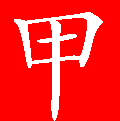
\includegraphics[width=3mm]{../Images/00002}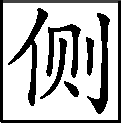
\includegraphics[width=3mm]{../Images/00011}\footnotesize \kaishu 阿凤活现纸上。}一面笑道:``老三还是这样慌脚鸡似的,我说你上不得高台板。赵姨娘时常也该教导教导他才是。''{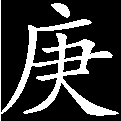
\includegraphics[width=3mm]{../Images/00004}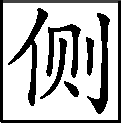
\includegraphics[width=3mm]{../Images/00011}\footnotesize \kaishu 为下文紧一步。}一句话提醒了王夫人,王夫人便不骂贾环,便叫过赵姨娘来骂道:``养出这样不知道理、下流黑心种子来,也不管管!几番几次我都不理论,{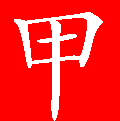
\includegraphics[width=3mm]{../Images/00002}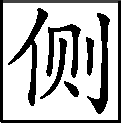
\includegraphics[width=3mm]{../Images/00011}\footnotesize \kaishu 补出素日来。}你们倒得了意了,这不益发上来了!''

那赵姨娘素日虽然也常怀嫉妒之心,不忿凤姐宝玉两个,也不敢露出来;如今贾环又生了事,受这场恶气,不但吞声承受,而且还要替宝玉来收拾。只见宝玉左边脸上烫了一溜燎泡,幸而眼睛没动。王夫人看了,又是心疼,又怕明日贾母问怎么回答,急的又把赵姨娘数落一顿。{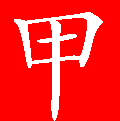
\includegraphics[width=3mm]{../Images/00002}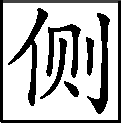
\includegraphics[width=3mm]{../Images/00011}\footnotesize \kaishu 总是为楔紧``五鬼''一回文字。}然后又安慰了宝玉一回,又命取败毒消肿药来敷上。宝玉道:``有些疼,还不妨事。明儿老太太问,就说是我自己烫的罢了。''凤姐笑{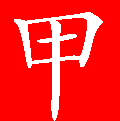
\includegraphics[width=3mm]{../Images/00002}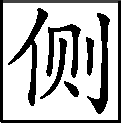
\includegraphics[width=3mm]{../Images/00011}\footnotesize \kaishu 两笑,坏极。 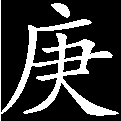
\includegraphics[width=3mm]{../Images/00004}\includegraphics[width=3mm]{../Images/00010}\footnotesize \kaishu 为五鬼法作引,非泛文也。雨窗。}道:``便说自己烫的,{\includegraphics[width=3mm]{../Images/00002}\includegraphics[width=3mm]{../Images/00011}\footnotesize \kaishu 玉兄自是悌弟之心性,一叹。}也要骂人为什么不小心看着,叫你烫了!横竖有一场气生,到明儿凭你怎么说去罢。''{\includegraphics[width=3mm]{../Images/00002}\includegraphics[width=3mm]{../Images/00011}\footnotesize \kaishu 坏极!总是调唆口吻,赵氏宁不觉乎?}王夫人命人好生送了宝玉回房,袭人等见了,都慌的了不得。

林黛玉见宝玉出了一天门,就觉得闷闷的,没个可说话的人。至晚正打发人来问了两三遍回来没有,这遍方才说回来,偏生又烫了脸。林黛玉便赶着来瞧,只见宝玉正拿镜子照呢,左边脸上满满的敷着一脸药。黛玉只当烫的十分利害,忙上来问怎么烫了,要瞧瞧。宝玉见他来了,忙把脸遮着,摇手不肯叫他看。知道他的癖性喜洁,见不得这些东西。{\includegraphics[width=3mm]{../Images/00002}\includegraphics[width=3mm]{../Images/00012}\footnotesize \kaishu 写宝玉文字,此等方是正经笔墨。}林黛玉自己也知道有这件癖性,{\includegraphics[width=3mm]{../Images/00002}\includegraphics[width=3mm]{../Images/00012}\footnotesize \kaishu 写林黛玉文字,此等方是正经笔墨。故二人文字虽多,如此等暗伏淡写处亦不少,观者实实看不出。}知道宝玉的心内怕他嫌脏,{\includegraphics[width=3mm]{../Images/00002}\includegraphics[width=3mm]{../Images/00011}\footnotesize \kaishu 二人纯用体贴功夫。 \includegraphics[width=3mm]{../Images/00002}\includegraphics[width=3mm]{../Images/00012}\footnotesize \kaishu 将二人一并,真真写他二人之心玲珑七窍。}因笑道:``我瞧瞧烫了那里了,有什么遮着藏着的。''一面说,一面就凑上来,强搬着脖子瞧了一瞧,问疼的怎么样。宝玉道:``也不很疼,养一两日就好了。''黛玉坐了一回,闷闷的回房去了。一宿无话。次日,宝玉见了贾母,虽然自己承认是自己烫的,不与别人相干,免不得贾母又把跟从的人骂一顿。{\includegraphics[width=3mm]{../Images/00002}\includegraphics[width=3mm]{../Images/00011}\footnotesize \kaishu 此原非正文,故草草写来。}

过了一日,就有宝玉寄名的干娘马道婆进荣国府来请安。见了宝玉,唬了一跳,问起原故,说是烫的,便点头叹惜一回,又向宝玉脸上用指头画了几画,又口内嘟嘟囔囔的持诵了一回,就说道:``管保你好了,这不过是一时飞灾。''又向贾母道:``祖宗老菩萨,那里知道那经典佛法上说的利害。{\includegraphics[width=3mm]{../Images/00002}\includegraphics[width=3mm]{../Images/00011}\footnotesize \kaishu 一段无伦无理信口开河的浑话,却句句都是耳闻目睹者,并非杜撰而有。作者与余实实经过。}大凡那王公卿相人家的子弟,只一生下来,暗中就有许多促狭鬼跟着他,得空便拧他一下,掐一下,或吃饭时打下他的饭碗来,或走着推他一跤,所以往往的那大家子的子孙多有长不大的。''贾母听见如此说,便赶着问:``这可有什么佛法解释没有呢?''马道婆道:``这个容易,只是替他多多作些因果善事也就罢了。再那经上还说,西方有位大光明普照菩萨,专管照耀阴暗邪祟,若有那善男子善女人虔心供奉者,可以永佑儿孙康宁安静,再无惊恐邪祟撞客之灾。''贾母道:``倒不知怎么供奉这位菩萨呢?''马道婆道:``也不值什么,除香烛供养之外,一天多使几斤香油,添在大海灯里。这海灯,就是菩萨的现身法像,昼夜是不敢熄的。''贾母道:``一天一夜也得多少油?明白告诉我,我好作这件功德。''马道婆听说,便笑道:``这也不拘,随施主们心愿舍罢了。像我们庙里,就有好几处的王妃诰命供奉:南安郡王太妃有许多,愿心大\href{../Text/part0029_split_000.html\#lnkback_2_a}{\textsuperscript{②}},{\includegraphics[width=3mm]{../Images/00002}\includegraphics[width=3mm]{../Images/00011}\footnotesize \kaishu 贼婆先用大铺排试之。}一天是四十八斤油,一斤灯草,那海灯也只比缸略小些;锦田侯的诰命次一等,一天不过二十四斤;再还有几家,也有五斤的、三斤的、一斤的,都不拘数。那小家子舍不起这些,就是四两半斤,也少不得替他点。''贾母听了,点头思忖。{\includegraphics[width=3mm]{../Images/00002}\includegraphics[width=3mm]{../Images/00010}\footnotesize \kaishu ``点头思忖''是量事之大小,非吝啬也。{[}壬午夏雨窗,畸笏。{]}◇日费香油四十八斤,每月油二百五十馀斤,合钱三百馀串。}\href{../Text/part0029_split_000.html\#lnkback_3_a}{\textsuperscript{③}}{为一小儿,如何服众?太君细心若是。}马道婆又道:``还有一件,若是为父母尊亲长上点,多舍些不妨;像老祖宗如今为宝玉,若舍多了倒不好,{\includegraphics[width=3mm]{../Images/00002}\includegraphics[width=3mm]{../Images/00011}\footnotesize \kaishu 贼道婆!是自``太君思忖''上来,后用如此数语收之,使太君必心悦诚服愿行。贼婆,贼婆,费我作者许多心机摹写也。}还怕他禁不起,倒折了福,也不当家。要舍,大则七斤,小则五斤,也就是了。''贾母说:``既这样,你便一日五斤合准了,每月来打趸关了去。''马道婆念了一声``阿弥陀佛,慈悲大菩萨''。贾母又命人来吩咐道:``以后大凡宝玉出门的日子,拿几串钱交给他小子们带着,遇见僧道穷苦之人好施舍的。''说毕,那马道婆又坐了一回,便又往各院各房问安,闲逛了一回。

一时来至赵姨娘房内,{\includegraphics[width=3mm]{../Images/00002}\includegraphics[width=3mm]{../Images/00011}\footnotesize \kaishu 有``各院各房'',接此方不觉突然。}二人见过,赵姨娘叫小丫头倒了茶来与他吃。马道婆因见炕上堆着些零碎绸缎弯角,赵姨娘正粘鞋呢。马道婆道:``可是我正没有鞋面子。{\includegraphics[width=3mm]{../Images/00002}\includegraphics[width=3mm]{../Images/00011}\footnotesize \kaishu 见者有分是也。}赵奶奶你有零碎缎子,不拘什么颜色,弄一双给我。''赵姨娘听说,叹口气道:``你瞧瞧,那里头还有那一块是成样的?成样的东西,也到不了我手里来!有的没的都在那里,你不嫌,就挑两块子去。''那马道婆见说,果真挑了两块袖起来。

赵姨娘问道:``可是前儿我送了五百钱去,在药王跟前上供,你可收了没有?''马道婆道:``早已替你上了供了。''赵姨娘叹口气道:``阿弥陀佛!我手里但凡从容些,也时常的上个供,只是心有馀力量不足。''马道婆道:``你只放心,将来熬的环哥儿大了,得个一官半职,那时你要做多大的功德不能?''赵姨娘听了,鼻子里笑了一声,道:``罢,罢,再别说起。如今就是个样儿,我们娘儿们跟的上那一个?也不是有了宝玉,竟是得了个活龙。他还是小孩子家,长的得人意儿,大人偏疼他些也还罢了;{\includegraphics[width=3mm]{../Images/00002}\includegraphics[width=3mm]{../Images/00011}\footnotesize \kaishu 赵妪数语,可知玉兄之身份,况在背后之言。}我只不服这个主儿。''{\includegraphics[width=3mm]{../Images/00002}\includegraphics[width=3mm]{../Images/00011}\footnotesize \kaishu 活现赵妪。}一面说,一面又伸出俩指头来。{\includegraphics[width=3mm]{../Images/00002}\includegraphics[width=3mm]{../Images/00011}\footnotesize \kaishu 活现阿凤。}马道婆会意,便问道:``可是琏二奶奶么?''赵姨娘唬的忙摇手儿,走到门前,掀帘子向外看看无人,{\includegraphics[width=3mm]{../Images/00002}\includegraphics[width=3mm]{../Images/00011}\footnotesize \kaishu 是心胆俱怕破。}方进来向马道婆悄悄的说道:``了不得,了不得!提起这个主儿,\href{../Text/part0029_split_000.html\#lnkback_4_a}{\textsuperscript{④}}这一分家私要不教他搬送了娘家去,我就不是个人。''{\includegraphics[width=3mm]{../Images/00004}\includegraphics[width=3mm]{../Images/00011}\footnotesize \kaishu 这是妒心正题目。}

马道婆见他如此说,便探他口气说道:\href{../Text/part0029_split_000.html\#lnkback_5_a}{\textsuperscript{⑤}}{\includegraphics[width=3mm]{../Images/00004}\includegraphics[width=3mm]{../Images/00011}\footnotesize \kaishu 有隙即入,所谓贼婆,是极!}``我还用你说,难道都看不出来?也亏你们心里都不理论,只凭他去。倒也妙。''赵姨娘道:``我的娘,不凭他去,难道谁还敢把他怎么样?''马道婆听说,鼻子里一笑,{\includegraphics[width=3mm]{../Images/00004}\includegraphics[width=3mm]{../Images/00011}\footnotesize \kaishu 二笑。}半晌说道:``不是我说句造孽的话,你们没本事也难怪。明不敢怎么样,暗里也就算计了,{\includegraphics[width=3mm]{../Images/00002}\includegraphics[width=3mm]{../Images/00011}\footnotesize \kaishu 贼婆操必胜之券,赵妪已堕术中,故敢直出明言。可畏可怕!}还等到这时候!''赵姨娘听这话有道理,心里暗暗的欢喜,便问道:``怎么暗里算计?我倒有这心,只是没这样的能干人。你若教给我这法子,我大大的谢你。''马道婆听说,这话打拢了一处,他便又故意说道:``阿弥陀佛!你快休问我,我那里知道这些事。罪过,罪过。''{\includegraphics[width=3mm]{../Images/00002}\includegraphics[width=3mm]{../Images/00011}\footnotesize \kaishu 远一步却是近一步。贼婆,贼婆!}赵姨娘道:``又来了。你是最肯济困扶危的人,难道就眼睁睁的看着人家来摆布死了我们娘儿两个不成?还是怕我不谢你?''马道婆听如此说,便笑道:``若说我不忍叫你娘儿们受了委屈还犹可,若说`谢'的这个字,可是你错打了法马了。就便是我希图你的谢,靠你又有什么东西能打动了我?''{\includegraphics[width=3mm]{../Images/00002}\includegraphics[width=3mm]{../Images/00011}\footnotesize \kaishu 探谢礼大小是如此说法,可怕可畏!}赵姨娘听这话口气松了些,便说道:``你这么个明白人,怎么也糊涂起来了。你若果然法子灵验,把他两个绝了,明日这家私不怕不是我环儿的。那时你要什么不得?''马道婆听说,低了头,半晌说道:``那时候事情妥当了,又无凭据,你还理我呢!''赵姨娘道:``这有何难。如今我虽手里没什么,也零零碎碎攒了几两梯己,还有几件衣服、簪子,你先拿了去。下剩的,我写个欠银子的文契给你,你要什么保人也有,到那时我照数给你。''马道婆道:``果然这样?''赵姨娘道:``这如何撒得谎!''说着便叫过一个心腹婆子来,在耳根底下嘁嘁喳喳说了几句话。{\includegraphics[width=3mm]{../Images/00002}\includegraphics[width=3mm]{../Images/00011}\footnotesize \kaishu 所谓狐群狗党,大家难免,看官着眼。}那婆子出去了,一时回来,果然写了个五百两的欠契来。赵姨娘便印了手模,{\includegraphics[width=3mm]{../Images/00002}\includegraphics[width=3mm]{../Images/00011}\footnotesize \kaishu 痴妇,痴妇!}走到厨柜里将梯己拿了出来,与马道婆看看,道:``这个你先拿了去,做香烛供奉使费,可好不好?''马道婆看看白花花的一堆银子,又有欠契,并不顾青红皂白,{\includegraphics[width=3mm]{../Images/00002}\includegraphics[width=3mm]{../Images/00011}\footnotesize \kaishu 有道婆作干娘者来看此句。``并不顾''三字怕杀人。千万件恶事皆从三字生出来。可怕可畏可警,可长存,戒之。}满口里应着,伸手先去接了银子掖起来,然后收了欠契。又向裤腰里掏了半晌,掏出十几个纸铰的青脸红发的鬼来,并两个纸人,{\includegraphics[width=3mm]{../Images/00002}\includegraphics[width=3mm]{../Images/00011}\footnotesize \kaishu 如此现成,更可怕。 \includegraphics[width=3mm]{../Images/00004}\includegraphics[width=3mm]{../Images/00011}\footnotesize \kaishu 如此现成,想贼婆所害之人岂止宝玉、阿凤二人哉?大家太君夫人诫之慎之。}递与赵姨娘,又悄悄的道:``把他两个的年庚八字写在这两个纸人身上,一并五个鬼都掖在他们各人的床上就完了。我只在家里作法,自有效验。千万小心,不要害怕!''{\includegraphics[width=3mm]{../Images/00002}\includegraphics[width=3mm]{../Images/00010}\footnotesize \kaishu 宝玉乃贼婆之寄名儿,{[}一样下此毒手,{]}况阿凤乎?三姑六婆之为害如此,即贾母之神明,在所不免。其他只知吃斋念佛之夫人太君,岂能防范得来?此{[}系老太君一大病。{]}作者一片婆心,不避嫌疑,特为写出,使看官再四着眼。吾家儿孙慎之戒之!}正才说完,只见王夫人的丫鬟进来找道:``奶奶可在这里,太太等你呢。''二人方散了,不在话下。

却说黛玉因见宝玉近日烫了脸,总不出门,倒时常在一处说说话儿。这日饭后看了二三篇书,自觉无味,便同紫鹃、雪雁做了一回针线,更觉得烦闷。便倚着房门出了一回神,{\includegraphics[width=3mm]{../Images/00002}\includegraphics[width=3mm]{../Images/00011}\footnotesize \kaishu 所谓``闲倚绣房吹柳絮''是也。}信步出来,看阶下新迸出的稚笋,{\includegraphics[width=3mm]{../Images/00002}\includegraphics[width=3mm]{../Images/00011}\footnotesize \kaishu 妙妙!``笋根稚子无人见'',今得颦儿一见,何幸如之。}不觉出了院门。一望园中,四顾无人,{\includegraphics[width=3mm]{../Images/00002}\includegraphics[width=3mm]{../Images/00011}\footnotesize \kaishu 恐冷落园亭花柳,故有是十数字也。}惟见花光柳影,鸟语溪声。{\includegraphics[width=3mm]{../Images/00002}\includegraphics[width=3mm]{../Images/00011}\footnotesize \kaishu 纯用画家笔写。}林黛玉信步便往怡红院来,只见几个丫头舀水,都在回廊上围着看画眉洗澡呢。{\includegraphics[width=3mm]{../Images/00002}\includegraphics[width=3mm]{../Images/00011}\footnotesize \kaishu 闺中女儿乐事。}听见房内有笑声,林黛玉便入房中看时,原来是李宫裁、凤姐、宝钗都在这里呢,一见他进来,都笑道:``这不又来了一个。''林黛玉笑道:``今日齐全,倒像谁下帖子请来的。''凤姐道:``前儿我打发人送了两瓶茶叶去,{\includegraphics[width=3mm]{../Images/00004}\includegraphics[width=3mm]{../Images/00011}\footnotesize \kaishu 有照应。}你往那去了?''黛玉笑道:``哦,可是我倒忘了,{\includegraphics[width=3mm]{../Images/00002}\includegraphics[width=3mm]{../Images/00011}\footnotesize \kaishu 该云``我正看《会真记》呢''。一笑。}多谢多谢。''凤姐又道:``你尝了可还好不好?''没有说完,宝玉便道:``论理可倒罢了,只是我说不大甚好,可也不知别人尝着怎么样。''宝钗道:``味倒轻,只是颜色不大很好。''{\includegraphics[width=3mm]{../Images/00004}\includegraphics[width=3mm]{../Images/00010}\footnotesize \kaishu 二宝答言,是补出诸艳俱领过之文。乙酉冬,雪窗。畸笏老人。}凤姐道:``那是暹罗进贡来的。我尝着也没什么趣儿,还不如我每日吃的呢。''黛玉道:``我吃着好。{\includegraphics[width=3mm]{../Images/00002}\includegraphics[width=3mm]{../Images/00011}\footnotesize \kaishu 卿爱因味轻也。卿如何担的起味厚之物耶?}''宝玉道:``你果然吃着好,把我这个也拿了去罢。''凤姐道:``你真爱吃,我那里还有呢。''林黛玉道:``果真的,我就打发人取去了。''凤姐道:``不用取去,我叫人送来就是了。我明日还有一件事求你,一同打发人送来。''黛玉听了笑道:``你们听听,这是吃了他一点子茶叶,就来使唤我来了。''凤姐笑道:``倒求你,你倒说这些闲话。你既吃了我们家的茶,怎么还不给我们家作媳妇?''{{\includegraphics[width=3mm]{../Images/00002}\includegraphics[width=3mm]{../Images/00011}\footnotesize \kaishu 二玉事,在贾府上下诸人,即看书人、批书人皆信定一{(段)}{[}双{]}好夫妻,书中常常每每道及。岂其不然,叹叹! \includegraphics[width=3mm]{../Images/00004}\includegraphics[width=3mm]{../Images/00011}\footnotesize \kaishu 二玉之配偶,在贾府上下诸人,即观者、批者、作者皆为无疑,故常常有此等点题语。}}众人听了都一齐笑起来。{\includegraphics[width=3mm]{../Images/00004}\includegraphics[width=3mm]{../Images/00011}\footnotesize \kaishu 我也要笑。}

黛玉便红了脸,一声儿也不言语,回过头去了。李宫裁笑向宝钗道:``真真我们二婶子的诙谐是好的。''{\includegraphics[width=3mm]{../Images/00004}\includegraphics[width=3mm]{../Images/00011}\footnotesize \kaishu 好赞!该他赞。}林黛玉含羞笑道:``什么诙谐,不过是贫嘴贱舌讨人厌恶罢了。''{\includegraphics[width=3mm]{../Images/00002}\includegraphics[width=3mm]{../Images/00011}\footnotesize \kaishu 此句还要候查。}说着便啐了一口。凤姐笑道:``你别作梦!给我们家作了媳妇,你想想------''便指宝玉道:``你瞧,人物儿、门第配不上,{\includegraphics[width=3mm]{../Images/00002}\includegraphics[width=3mm]{../Images/00011}\footnotesize \kaishu 大大一泄,好接后文。}还是根基配不上?模样儿配不上,是家私配不上?那一点玷辱了谁呢?''林黛玉便起身要走。宝钗便叫道:``颦儿急了,还不回来坐着。走了倒没意思。''说着便站起来拉住。

只见赵姨娘和周姨娘两个人进来瞧宝玉。李宫裁、宝钗、宝玉等都让他两个坐。独凤姐只和黛玉说笑,正眼也不看他们。宝钗方欲说话时,只见王夫人房内的丫头来说:``舅太太来了,请姑娘奶奶们出去呢。''李宫裁听了,忙叫着凤姐等要走。周、赵两个也忙辞了宝玉出去。宝玉道:``我也不能出去,你们好歹别叫舅母进来。''又道:``林妹妹,你先站一站,我和你说一句话。''凤姐听了,回头向黛玉笑道:``有人叫你说话呢。''说着,便把林黛玉往里一推,和李纨一同去了。

这里宝玉拉着林黛玉的袖子,只是嘻嘻的笑,{\includegraphics[width=3mm]{../Images/00004}\includegraphics[width=3mm]{../Images/00011}\footnotesize \kaishu 此刻好看之至!}心里有话,只是口里说不出来。{\includegraphics[width=3mm]{../Images/00002}\includegraphics[width=3mm]{../Images/00011}\footnotesize \kaishu 是已受镇说不出来,勿得错会了意。}此时林黛玉只是禁不住把脸红涨起来了,挣着要走。宝玉忽然``嗳哟''了一声,说:``好头疼!''{\includegraphics[width=3mm]{../Images/00002}\includegraphics[width=3mm]{../Images/00011}\footnotesize \kaishu 自黛玉看书起分三段写来,真无容针之空。如夏日乌云四起,疾闪长雷不绝,不知雨落何时,忽然霹雳一声,倾盆大注,何快如之,何乐如之,其令人宁不叫绝!}林黛玉道:``该,阿弥陀佛!''{\includegraphics[width=3mm]{../Images/00004}\includegraphics[width=3mm]{../Images/00010}\footnotesize \kaishu 黛玉念佛,是吃茶之语在心故也。然摹写神妙,一丝不漏如此。己卯冬夜。}只见宝玉大叫一声:``我要死!''将身一纵,离地跳有三四尺高,嘴里乱嚷乱叫,说起胡话来了。林黛玉并丫头们都唬慌了,忙去报知贾母、王夫人等。此时王子腾的夫人也在这里,都一齐来看时,宝玉越发拿刀弄杖,寻死觅活的。贾母、王夫人见了,唬的抖衣乱颤,且``儿''一声``肉''一声恸哭起来。于是惊动众人,连贾赦、邢夫人、贾珍、贾政、贾琏、贾蓉、贾芸、贾萍、薛姨妈、薛蟠并家中一干家人,上上下下里里外外众媳妇丫头等,都来园内看视。登时乱麻一般。{\includegraphics[width=3mm]{../Images/00002}\includegraphics[width=3mm]{../Images/00011}\footnotesize \kaishu 写玉兄惊动若许人忙乱,正写太君一人之钟爱耳。看官勿被作者瞒过。}正都没个主见,只见凤姐儿手持一把明晃晃钢刀砍进园来,见鸡杀鸡,见狗杀狗,见人就要杀人。{\includegraphics[width=3mm]{../Images/00002}\includegraphics[width=3mm]{../Images/00012}\footnotesize \kaishu 此处焉用鸡犬?然辉煌富丽,非处家之常也,鸡犬闲闲,始为儿孙千年之业,故于此处必用``鸡犬''二字,方是一簇腾腾大舍。}众人越发慌了。周瑞媳妇忙带着几个有力量的胆壮的婆娘上去抱住,夺下刀来,抬回房去。平儿、丰儿等哭的泪天泪地。贾政等心中也有些烦难,顾了这里,丢不下那里。

别人慌张自不必讲,独有薛蟠更比诸人忙到十分去:{\includegraphics[width=3mm]{../Images/00002}\includegraphics[width=3mm]{../Images/00011}\footnotesize \kaishu 写呆兄忙,是愈觉忙中之愈忙,且避正文之絮烦。好笔仗,写得出。 \includegraphics[width=3mm]{../Images/00004}\includegraphics[width=3mm]{../Images/00011}\footnotesize \kaishu 写呆兄忙是躲烦碎文字法。好想头,好笔力。《石头记》最得力处在此。}又恐薛姨妈被人挤倒,又恐薛宝钗被人瞧见,又恐香菱被人臊皮------知道贾珍等是在女人身上做工夫的,{\includegraphics[width=3mm]{../Images/00002}\includegraphics[width=3mm]{../Images/00011}\footnotesize \kaishu 从阿呆兄意中,又写贾珍等一笔,妙!}因此忙的不堪。忽一眼瞥见了林黛玉风流婉转,已酥倒在那里。{\includegraphics[width=3mm]{../Images/00002}\includegraphics[width=3mm]{../Images/00011}\footnotesize \kaishu 忙到容针不能。此似唐突颦儿,却是写情字万不能禁止者,又可知颦儿之丰神若仙子也。 \includegraphics[width=3mm]{../Images/00002}\includegraphics[width=3mm]{../Images/00012}\footnotesize \kaishu 忙中写闲,真大手眼,大章法。}

当下众人七言八语,有的说请端公送祟的,有的说请巫婆跳神的,有的又荐什么玉皇阁的张真人,种种喧腾不一。也曾百般的医治祈祷,问卜求神,总无效验。堪堪的日落。王子腾的夫人告辞去后,次日王子腾自己亲来瞧问。{\includegraphics[width=3mm]{../Images/00002}\includegraphics[width=3mm]{../Images/00011}\footnotesize \kaishu 写外戚,亦避正文之繁。}接着小史侯家、邢夫人兄弟辈并各亲眷都来瞧看,也有送符水的,也有荐僧道的,也都不见效。他叔嫂二人越发糊涂,不省人事,睡在床上,浑身火炭一般,口内无般不说。到夜时,那些婆娘、媳妇、丫头们都不敢上前。因此把他二人都抬到王夫人的上房内,{\includegraphics[width=3mm]{../Images/00002}\includegraphics[width=3mm]{../Images/00011}\footnotesize \kaishu 收拾得干净有着落。 \includegraphics[width=3mm]{../Images/00004}\includegraphics[width=3mm]{../Images/00011}\footnotesize \kaishu 收拾的得体正大。}夜间派了贾芸等带着小子们挨次轮班看守。贾母、王夫人、邢夫人、薛姨妈等寸地不离,只围着干哭。

此时贾赦、贾政又恐哭坏了贾母,日夜熬油费火,闹的人口不安,也都没有主意。贾赦还是各处去寻僧觅道。贾政见都不灵效,着实懊恼,{\includegraphics[width=3mm]{../Images/00002}\includegraphics[width=3mm]{../Images/00011}\footnotesize \kaishu 四字写尽政老矣。}因阻贾赦道:``儿女之数,皆由天命,非人力可强者。他二人之病出于不意,百般医治不效,想天意该当如此,也只好由他们去罢。''{\includegraphics[width=3mm]{../Images/00002}\includegraphics[width=3mm]{../Images/00011}\footnotesize \kaishu 念书人自应如是语。}贾赦也不理此话,仍是百般忙乱,那里见些效验。看看三日光阴,那凤姐和宝玉躺在床上,一发连气都将没了。合家人口无不惊慌,都说没了指望,忙着将他二人的后世衣履都治备下了。贾母、王夫人、贾琏、平儿、袭人这几个人,更比诸人哭的忘餐废寝,觅死寻活。赵姨娘、贾环等心中欢喜称愿。{\includegraphics[width=3mm]{../Images/00002}\includegraphics[width=3mm]{../Images/00011}\footnotesize \kaishu 补明赵妪进怡红为作法也。}

到了第四日早晨,贾母等正围着他两个哭时,只见宝玉睁开眼说道:{\includegraphics[width=3mm]{../Images/00002}\includegraphics[width=3mm]{../Images/00011}\footnotesize \kaishu ``语不惊人死不休'',此之谓也。}``从今以后,我可不在你家了!快些收拾,打发我走罢。''贾母听了这话,就如同摘去心肝一般。赵姨娘在旁劝道:``老太太也不必过于悲痛了。{\includegraphics[width=3mm]{../Images/00004}\includegraphics[width=3mm]{../Images/00011}\footnotesize \kaishu 断不可少此句。}哥儿已是不中用了,不如把哥儿的衣裳穿好,让他早些回去罢,也免些苦。只管舍不得他,这口气不断,他在那世里也受罪不安生。''{\includegraphics[width=3mm]{../Images/00004}\includegraphics[width=3mm]{../Images/00011}\footnotesize \kaishu 大遂心人必有是语。}这些话还没说完,被贾母照脸啐了一口唾沫,骂道:``烂了舌根的混帐老婆,谁叫你来多嘴多舌的!你怎么知道他在那世里受罪不安生?怎么见得不中用了?你愿他死了,有什么好处?你别做梦!他死了,我只和你们要命。素日都是你们调唆着逼他写字念书,{\includegraphics[width=3mm]{../Images/00002}\includegraphics[width=3mm]{../Images/00012}\footnotesize \kaishu 奇语,所谓溺爱者不明,然天生必有是一段文字的。}把胆子唬破了,见了他老子还不像个避猫鼠儿?都不是你们这起淫妇调唆的!这会子逼死了他,你们遂了心了。我饶那一个!''一面骂,一面哭。贾政在旁听见这些话,心中越发难过,便喝退赵姨娘,自己上来委婉解劝。一时又有人来回说:``两口棺材都作齐备了,{\includegraphics[width=3mm]{../Images/00002}\includegraphics[width=3mm]{../Images/00011}\footnotesize \kaishu 偏写一头不了又一头之文,真步步紧之文。}请老爷出去看。''贾母听了,如火上浇油一般,便骂道:``是谁做了棺材?''一叠连声只叫把做棺材的拉来打死。

正闹的天翻地覆,没个开交,只闻得隐隐的木鱼声响,{\includegraphics[width=3mm]{../Images/00002}\includegraphics[width=3mm]{../Images/00011}\footnotesize \kaishu 不费丝毫勉强,轻轻收住数百言文字,《石头记》得力处全在此处。以幻作真,以真作幻,看书人亦要如是看法为幸。}念了一句:``南无解冤孽菩萨。''又听说道:``有那人口不安,家宅颠倾,或逢凶险,或中邪祟不利者,我们善能医治。''贾母、王夫人等听见这些话,那里还耐得住,便命人去快请来。贾政虽不自在,奈贾母之言如何违拗;又想如此深宅,何得听的如此真切,{\includegraphics[width=3mm]{../Images/00002}\includegraphics[width=3mm]{../Images/00011}\footnotesize \kaishu 作者是幻笔,合屋俱是幻耳,焉能无闻?}心中亦是希罕,{\includegraphics[width=3mm]{../Images/00002}\includegraphics[width=3mm]{../Images/00011}\footnotesize \kaishu 政老亦落幻中。}便命人请了进来。众人举目看时,原来是一个癞头和尚与一个跛足道人。{\includegraphics[width=3mm]{../Images/00002}\includegraphics[width=3mm]{../Images/00012}\footnotesize \kaishu 僧因凤姐,道因宝玉,一丝不乱。}只见那和尚是怎生模样:

鼻如悬胆两眉长,目似明星蓄宝光,

破衲芒鞋无住迹,腌臜更有满头疮。

看那道人又是怎生模样,但见:

一足高来一足低,浑身带水又拖泥。

相逢若问家何处,却在蓬莱弱水西。

贾政问道:``你道友二人在那庙焚修?''那僧笑道:``长官不须多言。{\includegraphics[width=3mm]{../Images/00002}\includegraphics[width=3mm]{../Images/00011}\footnotesize \kaishu 避俗套法。}因闻得尊府人口不利,故特来医治。''贾政道:``倒有两个人中邪,不知二位有何符水?''那道笑道:``你家现放着希世奇珍,如何倒还问我们有符水?''贾政听这话有意思,心中便动了,因说道:``小儿落草时虽带了一块宝玉下来,上面说能除邪祟,{\includegraphics[width=3mm]{../Images/00004}\includegraphics[width=3mm]{../Images/00011}\footnotesize \kaishu 点题。}谁知竟不灵验。''那僧笑道:``长官,你那里知道那物的妙用。只因他如今被声色货利所迷,{\includegraphics[width=3mm]{../Images/00002}\includegraphics[width=3mm]{../Images/00012}\footnotesize \kaishu 石且能迷,可知其害不小。观者着眼,方可读《石头记》。 \includegraphics[width=3mm]{../Images/00004}\includegraphics[width=3mm]{../Images/00011}\footnotesize \kaishu 棒喝之声。}故此不灵验了。{\includegraphics[width=3mm]{../Images/00002}\includegraphics[width=3mm]{../Images/00011}\footnotesize \kaishu 读书者观之。}你今且取他出来,待我们持诵持诵,只怕就好了。''{\includegraphics[width=3mm]{../Images/00004}\includegraphics[width=3mm]{../Images/00011}\footnotesize \kaishu ``只怕''二字,是不知此石肯听持诵否?}

贾政听说,便向宝玉项上取下那玉来递与他二人。那和尚接了过来,擎在掌上,长叹一声道:``青埂峰一别,展眼已过十三载矣!{\includegraphics[width=3mm]{../Images/00004}\includegraphics[width=3mm]{../Images/00011}\footnotesize \kaishu 正点题,大荒山手捧时语。}人世光阴,如此迅速,尘缘满日,若似弹指!{\includegraphics[width=3mm]{../Images/00002}\includegraphics[width=3mm]{../Images/00012}\footnotesize \kaishu 见此一句,令人可叹可惊,不忍往后再看矣!}可羡你当时的那段好处:

天不拘兮地不羁,心头无喜亦无悲;{\includegraphics[width=3mm]{../Images/00002}\includegraphics[width=3mm]{../Images/00011}\footnotesize \kaishu 所谓越不聪明越快活。}

却因煅炼通灵后,便向人间觅是非。

可叹你今朝这番经历:

粉渍脂痕污宝光,绮栊昼夜困鸳鸯。

沉酣一梦终须醒,{\includegraphics[width=3mm]{../Images/00002}\includegraphics[width=3mm]{../Images/00011}\footnotesize \kaishu 无百年的筵席。}冤孽偿清好散场!''{\includegraphics[width=3mm]{../Images/00002}\includegraphics[width=3mm]{../Images/00011}\footnotesize \kaishu 三次煅炼,焉得不成佛作祖?}

念毕,又摩弄一回,说了些疯话,递与贾政道:``此物已灵,不可亵渎,悬于卧室上槛。将他二人安在一室之内,除亲身妻母外,不可使外人冲犯。{\includegraphics[width=3mm]{../Images/00004}\includegraphics[width=3mm]{../Images/00011}\footnotesize \kaishu 是要紧语,是不可不写之套语。}三十三天之后,包管身安病退,复旧如初。''说着,回头便走了。{\includegraphics[width=3mm]{../Images/00004}\includegraphics[width=3mm]{../Images/00010}\footnotesize \kaishu 通灵玉除邪,全部百回只此一见,何得再言?僧道踪迹虚实,幻笔幻想,写幻人于幻文也。壬午孟夏,雨窗。}贾政赶着,还说让他二人坐了吃茶,要送谢礼,他二人早已出去了。贾母等还只管使人去赶,那里有个踪影?少不得依言将他二人就安在王夫人卧室之内,将玉悬在门上。
王夫人亲自守着,不许别个人进来。

至晚间,他二人竟渐渐的醒来,{\includegraphics[width=3mm]{../Images/00002}\includegraphics[width=3mm]{../Images/00011}\footnotesize \kaishu 能领持诵,故如此灵效。}说腹中饥饿。贾母、王夫人等如得了珍宝一般,{\includegraphics[width=3mm]{../Images/00002}\includegraphics[width=3mm]{../Images/00011}\footnotesize \kaishu 昊天罔极之恩如何报得?哭杀幼而丧亲者。}旋熬了米汤来与他二人吃了,精神渐长,邪祟少退,一家子才把心放下来。{\includegraphics[width=3mm]{../Images/00002}\includegraphics[width=3mm]{../Images/00010}\footnotesize \kaishu 通灵玉听癞和尚二偈即刻灵应,抵却前回若干《庄子》及语录机锋偈子。正所谓物各有所主也。◇叹不得见玉兄``悬崖撒手''文字为恨。{[}丁亥夏,畸笏叟。{]}}李宫裁并贾府三艳、薛宝钗、林黛玉、平儿、袭人等在外间听信。闻得吃了米汤,省了人事,别人未开口,林黛玉先就念了声``阿弥陀佛''。{\includegraphics[width=3mm]{../Images/00002}\includegraphics[width=3mm]{../Images/00011}\footnotesize \kaishu 针对得病时那一声。}宝钗便回头看了他半日,``嗤''的一笑。众人都不会意,惜春问道:``宝姐姐,好好的笑什么?''宝钗笑道:``我笑如来佛比人还忙:{\includegraphics[width=3mm]{../Images/00004}\includegraphics[width=3mm]{../Images/00011}\footnotesize \kaishu 这一句作正意看,馀皆雅谑,但此一谑抵颦儿半部之谑。}又要讲经说法,又要普渡众生;这如今宝玉与二姐姐病了,又是烧香还愿、赐福消灾;今儿才好些,又要管林姑娘的姻缘了。你说忙的可笑不可笑。''黛玉不觉红了脸,啐了一口道:``你们这起人不是好人,不知怎么死!再不跟着好人学,只跟那些贫嘴恶舌的人学。''一面说,一面摔帘子出去了。

\includegraphics[width=3mm]{../Images/00002}{总批:先写红玉数行引接正文,是不作开门见山文字。}

{灯油引``大光明普照菩萨'',``大光明普照菩萨''引五鬼魇魔法是一线贯成。}

{通灵玉除邪,全部只此一见,却又不灵,遇癞和尚、跛道人一点方灵应矣。写利欲之害如此。}

{此回本意是为禁三姑六婆进门之害,难以防范。}

{{\includegraphics[width=3mm]{../Images/00004}此回书因才干乖觉太露引出事来,作者婆心,为世之乖觉人为鉴。}}

{\includegraphics[width=3mm]{../Images/00005}总评:欲深魔重复何疑,苦海冤河解者谁?结不休时冤日盛,井天甚小性难移。}

{}

{\href{../Text/part0029_split_000.html\#navto_1_a}{①}原作``四'',庚、戚宁、蒙、列、舒本均同,当系早期原稿本之误。据有正、甲辰本改为``三'',杨本则改为``几''。}

{\href{../Text/part0029_split_000.html\#navto_2_a}{②}``有许多,愿心大'',文字有点别扭,意思还明白。其他各本改文也未见佳,不从。}

{\href{../Text/part0029_split_000.html\#navto_3_a}{③}此批折算月耗油量显误。有网友提出后一``斤''字应为``金''字音讹,为月耗油钱额。可参考。}

{\href{../Text/part0029_split_000.html\#navto_4_a}{④}此后列、杨本多出``来,真真把人气杀,叫人一言难尽。我白和你打个赌,明儿''22字,语气似更完整顺畅。但因庚、戚、蒙等本同无此语,当非底本夺漏,而是列、杨本擅增。}

{\href{../Text/part0029_split_000.html\#navto_5_a}{⑤}原只作``马道婆道'',亦通。为兼顾庚本批语,据诸本补。}
